\newpage

\section{Image Processing}\label{sec:image_processing}

\subsubsection{Definition of the object detection task}

The deep learning computer vision area consists of different tasks, which serve different purposes. In figure \ref{fig:object_detection} we can see the representation of these different tasks. In our project we will take a closer look on the object detection. Like we can see in the image, object detection means detecting multiple objects. But the task it not only to detect and classify them, it is also the task of the program to locate the objects. This will be evaluated on the bounding box around the object.  The desired result can be seen in the following figure.

\begin{figure}[H]
\centering
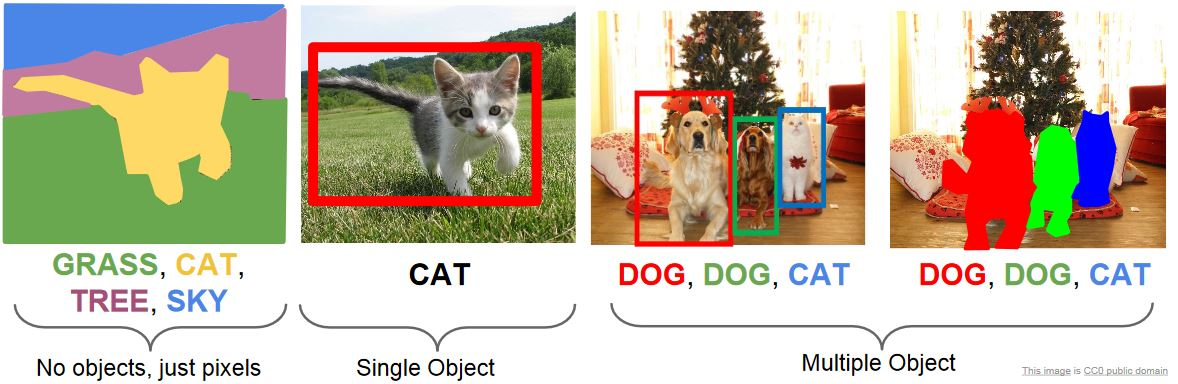
\includegraphics[width=\textwidth]{sources/object_detection.png}
\caption[Image processing task]{Representation of image processing tasks}
\label{fig:object_detection}
\end{figure}

\subsubsection{Requirements on object detection}

In our project we only define the object, which we want to detect. It is not defined how many of these objects will be present, but for the expandability of the project, we will use methods capable of detecting multiple objects.\\

Also, the image processing needs to be real-time capable. The robot navigates autonomously around an unknown area and should detect the objects, when they appear. It is not desirable to have delays in the detection. For this also a sufficient accuracy is needed to detect the object under different lighting and background conditions. \\

\subsection{Basic model selection}\label{subsec:basic_model_selection}

Regarding these requirements, we need a specialized model to match the real-time capabilities, while having a decent accuracy. In the image recognition area, the drive for increasing accuracy leads the progress. But it comes with the cost of increasing complexity of the models. This leads to increasing computational cost, which decrease the real-time capabilities. Mobile phones and embedded system are not capable of providing this performance. For this purpose, the MobileNet \cite{tim1} network was created. It drastically decreases the number of trainable parameters with different techniques. The main difference from conventional networks is the depthwise convolution. In the conventional convolutional network, the convolution determines features by applying kernel filters on the different input channels and combines the features to reach a new representation \cite{tim1}.\\

This results in a computational cost of:

$$ D_K \cdot D_K \cdot M \cdot N \cdot D_F \cdot D_F$$

The MobileNet splits these two steps up and computes them separately \cite{tim2,tim3}.  First the depthwise convolution is applied by applying a single filter per input channel. In the second step the pointwise convolution combines the resulting features. Both operations present an own layer and are followed by a batch normalization and a ReLU activation. This separation results in a new computational cost of:

$$ D_K \cdot D_K \cdot M \cdot D_F \cdot + M \cdot N \cdot D_F \cdot D_F $$

Comparing these to costs, the depthwise convolution reaches a reduction of $ \dfrac{1}{N} + \dfrac{1}{D^2_K} $.

\begin{figure}[H]
\centering
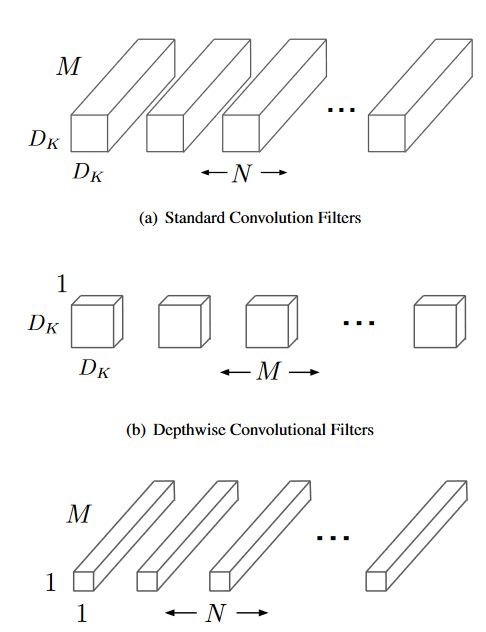
\includegraphics[scale=0.65]{sources/depthwise_convolution.JPG}
\caption[Comparison standard and depthwise]{Comparison of standard convolution (a) and Depthwise Convolution \cite{tim2,tim3}}
\label{fig:depthwise_convolution}
\end{figure}

The Mobile network was tested one time with standard convolution and with depthwise separable convolution. The result was only 1,1\,\% loss in accuracy, but a reduction of 25,1 million parameters. 

\begin{figure}[H]
\centering
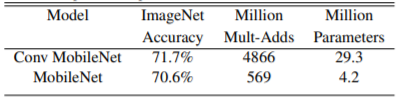
\includegraphics{sources/Comparison_Mobilenet.png}
\caption[Comparison standard and separable depthwise]{Comparison of standard and depthwise separable convolution}
\label{fig:depthwise_convolution}
\end{figure}

\subsection{Object Detection System}\label{subsec:object_detection_system}

For the object detection there are mainly three different techniques, which are used.

\subsubsection{Faster R-CNN}

One approach is the Faster R-CNN, which is the combination of two modules. First we have a deep convolutional network, which extracts the features. After this the feature map will be shared with a separate network, which predicts the region proposals. In this RPN module the feature map will be fed into two fully-connected layers. One layer computes the box regression and the other one computes the box classification. These predictions will be reshaped through a RoI (Region of Interest) pooling layer and will then be used to classify the found objects within the proposed regions.

\begin{figure}[H]
\centering
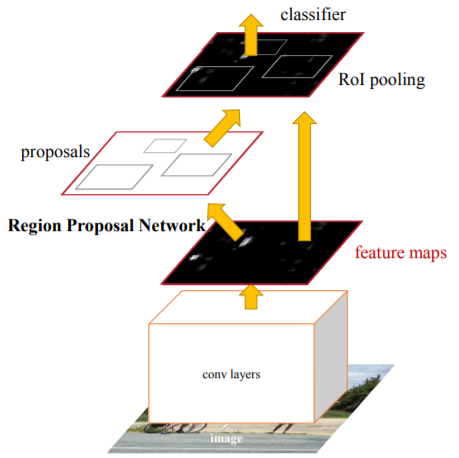
\includegraphics{sources/Faster_R-CNN.png}
\caption[Architecture of Faster R-CNN]{Architecture of Faster R-CNN \cite{tim2}}
\label{fig:depthwise_convolution}
\end{figure}

\subsubsection{You Only Look Once -- YOLO}

Another approach is to not look at regions with high probability of containing an object, but to split the whole image into a grid and predict first the class probability and secondly the offset for the bounding box for different bounding boxes in this grid. The only probabilities higher than a defined threshold will be taken into consideration. This reduces the architecture to one network and eliminates the bottleneck separate classification and bounding box regression. This approach is called YOLO (You Only Look Once), which is a lot faster than Faster R-CNN, but has the drawback of less accuracy \cite{tim3}.

\subsubsection{Single Shot Detection -- SSD}

The last approach uses the same technique as YOLO, but has some diversifications. Single Shot Detection (SSD) is also a one-stage detection model. It predicts class and bounding box at the same time. Unlike YOLO it will not predict the certainty of the object being an object, its only predicts the class probabilities, but adds a background class. So when thebackground class has a high probability, it has the same effect as a low confidence score from the YOLO prediction.\\

Also, the SSD uses different grid layouts, which results in more predictions, but also in more accuracy. Therefore, the YOLO architecture delivers better real-time capabilities, because is it less computational intense.

\begin{figure}[H]
\centering
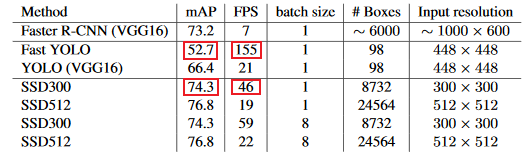
\includegraphics{sources/tempsnip.png}
\caption[Performance comparison of different techniques]{Performance comparison of different techniques \cite{tim5}}
\label{fig:depthwise_convolution}
\end{figure}

\subsection{Experiments}

For our object detection experiments we used the following software components:

\begin{itemize}
\itemsep0em
\item Python 3.7.3
\item OpenCV 4.1.2 \cite{tim6}
\item ImageZMQ \cite{tim7}
\item Imutils \cite{tim8}
\item ssd\_mobilenet\_v2\_coco \cite{tim9}
\end{itemize}

We used OpenCV, because it is a well-established computer vision library and designed for fast computation also on system with low computational capabilities. It offers the DNN (Deep Neural Network) module, which implements methods to import pretrained models from different frameworks. We decided to take the pretrained MobilenetV2 in combination with SSD trained on the COCO dataset. For reasons shown in Section \ref{subsec:object_detection_system}. and \ref{subsec:basic_model_selection}., we decided this network will give us enough computation speed to detect object while driving and sufficient accuracy to detect the object in different lighting or environment conditions. The COCO (Common Objects in Context) dataset is a commonly used dataset and offers a lot of classes. We defined the ``sports ball'' class as the desired object to detect but wanted to have flexibility to change the object if needed. Therefore, the COCO dataset was well-suited for our requirements.\\

The ``ImageZMQ'' package is a little library with methods to transport the OpenCV images over the network. It uses the ZeroMQ sockets to enable an easy and fast transport.\\

The ``imutils'' package is used to build up the presentation of the images.

\subsection{Software}

Because The images will be sent over network to an external device, two scripts will be started. One is the client script, which runs on the Raspberry Pi. The server script runs on the external device and receives and processes the images. It also sends the acknowledgement to signal the client to send another picture.

\begin{figure}[H]
\centering
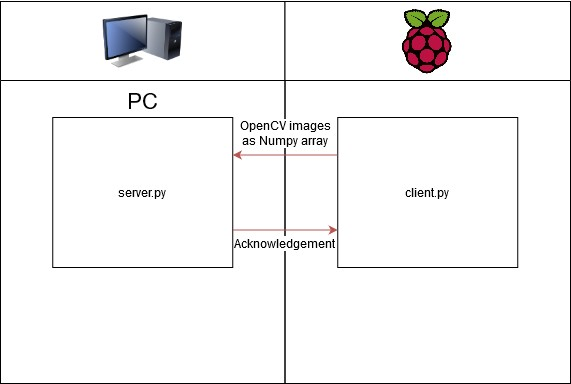
\includegraphics[scale=0.8]{sources/client_server.jpg}
\caption[Server client communication]{Server client communication}
\label{fig:depthwise_convolution}
\end{figure}

\subsubsection{Server.py}

The server first initializes the socket to receive the images and the connection to the ``Object\_hunt\_base'' process. Then the network will be initialized and the objects to consider.\\

The marker for a found object will be set to False before the loop. In the loop the image will be received if there is a connection. If the device is not already known, it will be added to the ``lastActive'' list. The image will be resized and then processed by the network.  If an detection of the desired object occurred and the confidence is higher than the defined threshold, the presentation will be build. The bounding box will be added to the picture and the number of detected objects will be updated. This image will then be shown on the external device. The loop is also interrupted and the connection to the object\_hunt\_base process will be established to send the message of successful object detection. Then the picture of detection will be shown, until the user interrupts the script.

\subsubsection{Client.py}

The client initializes the connection to the server and initializes the camera. In an endless loop the client will send the images to the server.

\subsection{Results}

We could realize all the requirements we set for our object detection task. Our project has shown, that for real-time object detection it is possible to let the image processing run on an external device and still get sufficient results. Our object detection is flexible in detecting different classes, it is possible to choose one of all COCO classes. To get better accuracy and better performance an own dataset will be needed. With an own dataset, the network would only predict two different classes, the background and the desired object, which result in much less predictions and therefore better performance.
